\clearpage
\section{Preliminaries}\label{sec:prel}

This section introduces notation and other preliminaries used in the remainder
of the specification.

\subsection{Notation}

The specification uses set-notation based approach while also inspired
by~\cite{eutxo-2}~and~\cite{eutxo}.\todo{handwavy} Values $a$ are of a set
$a \in \mathcal{A}$, also indicated as being of some type $a : \mathcal{A}$, and
complex values are tuples drawn from a $\times$ product of multiple sets, e.g.
$(a,b) \in (\mathcal{A} \times \mathcal{B})$. An empty set is indicated by
$\emptyset$. Sets may be enumerated using $\{\}$, the $=$ operator means
correspondence and $\gets$ is explicit assignment of a variable or value to one
or more variables. Functions are morphisms mapping from one to another set
$x : \mathcal{A} \to f(x) : \mathcal{B}$, where function
application of a function $f$ to an argument $x$ is written as $f(x)$. \\

% TODO: use ^* or FinSup for values?
% \noindent Given a set $\mathcal{A}$, let
% \begin{itemize}
%   \item $\mathcal{A}^0 = \mathcal{A} \cup \emptyset$,
%   \item $\mathcal{A}^n$ be the set of all n-sized sequences over $\mathcal{A}$,
%   \item $\mathcal{A}^! = \bigcup_{i=1}^{n \in \tyNatural} \mathcal{A}^{i}$, and
%   \item $\mathcal{A}^* = \bigcup_{i=0}^{n \in \tyNatural} \mathcal{A}^{i}$.
% \end{itemize}

\noindent Variables may have modifiers: when $x$ is a single value,
\begin{itemize}
  \item $x'$ is a modified value (but from same set / type),
  \item $\underline{x}$ is list of values,
  \item $\tilde{x}$ is an aggregated value, and
  \item $x^{\#}$ is the result of $\hash(x)$.
\end{itemize}

\noindent With this, we further define:
\begin{itemize}
  \item $\tyBool = \{\false, \true\}$ are boolean values
  \item $\tyNatural$ are natural numbers $\{0, 1, 2, \ldots\}$
  \item $\tyInteger$ are integer numbers $\{\ldots, −2, −1, 0, 1, 2, \ldots\}$
  \item $\tyBytes = \bigcup_{n=0}^{\inf}{\{0,1\}}^{8n}$ denotes a arbitrary
        string of bytes
  \item $\oplus : \tyBytes \to \tyBytes$ is concatenatenating bytes
  \item $\hash : x \to x^{\#}$ denotes a cryptographic collision-resistant
        hashing function
  \item $\bytes : x \to \tyBytes$ denotes an invertible serialisation function
        mapping arbitrary data to bytes
  \item Lists of values are written as $l = [x_{1}, \ldots, x_{n}]$. Empty lists
        are denoted by $[]$, the $i$th element $x_{i}$ is also written $l[i]$
        and the length of the list is $|l| = n$.
  \item $\tyData$ is a universal data type of nested sums and products built up
        recursively from the base types of $\tyInteger$ and $\tyBytes$.
\end{itemize}

\subsection{Public key cryptography and multi-signature scheme}\label{sec:multisig}

\todo{be specific!?}
% TODO: Not keep this generic and only specific (naiive) as it is right now?
A multisignature scheme~\cite{itakura1983public,CCS:MicOhtRey01}\todo{is this consistent with refs?} is a
tuple of algorithms:
\[
\ms \in (\msSetup \times \allowbreak\msKeyGen \times \allowbreak\msCombVK \times \allowbreak
\msSign \times \allowbreak\msComb \times \allowbreak\msVfy)
\]
Where $\msSetup$ generates public parameters $\msParams$, such that
\begin{itemize}
  \item $(\msVK,\msSK) \gets \msKeyGen(\msParams)$ can be used to generate fresh
        key pairs,
  \item $\msSig \gets \msSign(\msParams,\msSK,\msMsg)$ signs a message $\msMsg$
        using key $\msSK$,
  \item $\msCSig \gets \msComb(\msParams,\msMsg,\msVKL,\msSigL)$ aggregates
        \todo{requires a message?} a list $\msSigL$ of signatures into a single,
        aggregate signature~$\msCSig$.
  \item $\msCVK \gets \msCombVK(\msParams,\msVKL)$ aggregates a tuple\todo{set?}
        $\msVKL$ of verification keys into a single, aggregate key
        $\msCVK$\todo{difference $\msCVK$ vs. $\msVKL$?},
  \item $\msVfy(\msParams,\msCVK,\msMsg,\msCSig) \in \tyBool$ verifies an aggregate
        signature $\msCSig$ of message $\msMsg$ under an aggregate verification
        key $\msCVK$.
\end{itemize}

Note that in the following, we make the parameter~$\msParams$ implicit and leave
out the $ver$ suffix for verification key such that $k = k^{ver}$ for better
readability.

The security definition of a multisignature scheme
from~\cite{itakura1983public,CCS:MicOhtRey01} guarantees that, if $\msCVK$ is
produced from a tuple\todo{set?} of verification keys $\msVKL$ via $\msCombVK$,
then no aggregate signature $\msCSig$ can pass verification
$\msVfy(\msCVK,\msMsg,\msCSig)$ unless all honest parties holding keys in
$\msVKL$ signed $m$.

\subsection{Extended UTxO}\label{sec:eutxo}
The Hydra Head protocol is specified to work on the so-called Extended UTxO (EUTxO) ledgers
like Cardano.

The basis for EUTxO is is Bitcoin's UTxO ledger
model~\cite{formal-model-of-bitcoin-transactions,Zahnentferner18-UTxO}.
Intuitively, it arranges transactions in a directed acyclic graph, such as the
one in Figure~\ref{fig:utxo-graph}, where boxes represent transactions with
(red) inputs to the left and (black) outputs to the right. A dangling
(unconnected) output is an \emph{unspent transaction output (UTxO)} --- there
are two UTxOs in the figure.

\begin{figure}[h]
  \centering
 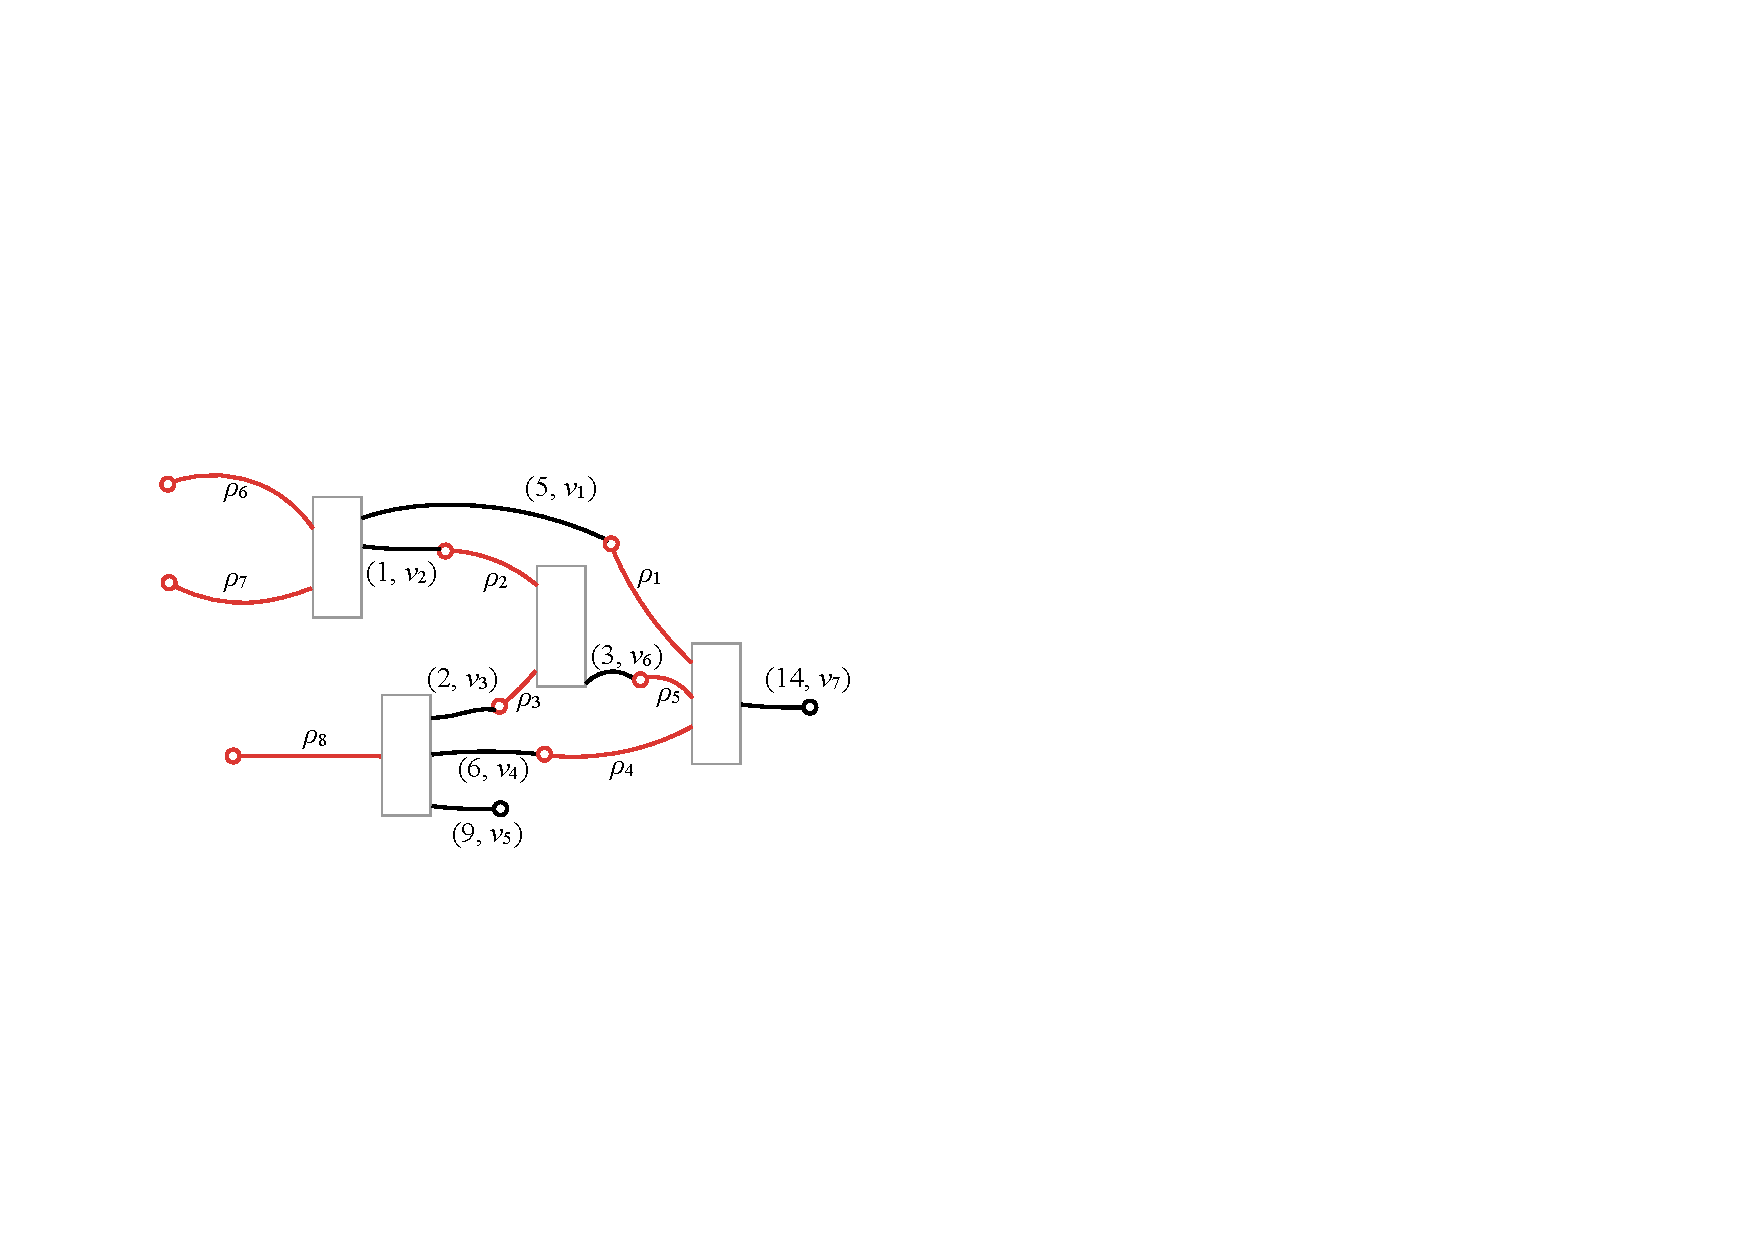
\includegraphics[width=\textwidth/2]{figures/utxo-graph.pdf}
 \caption{Example of a plain UTxO graph}\label{fig:utxo-graph}
\end{figure}

The following paragraphs will give definitions of the UTxO model and it's
extension to support scripting (EUTxO) suitable for this Hydra Head protocol
specification. For a more detailed introduction to the EUTxO ledger model,
see~\cite{eutxo},~\cite{eutxo-2}~and~\cite{utxo-ma}.

\begin{definition}[Values]
  Values are sets that keep track how many units of which tokens of which
  currency are available. Given a finitely supported function $\mapsto$, that
  maps keys to monoids, a value is the set of such mappings over a minting
  policy identifiers $\mathsf{pid}$, over a mapping of token names
  $\mathsf{tok}$ to quantities $q$:

  \[
    \val \in \tyValue = (\mathsf{pid} : \tyBytes \mapsto (\mathsf{tok} : \tyBytes \mapsto q : \tyInteger))
  \]

  Addition of values is defined as $+$, $\varnothing$ is the empty value,
  and \(\{t_1, \ldots, t_n\} :: c\) is used as a shorthand for
  \(\{c \mapsto \{t_1 \mapsto 1, \ldots, t_n \mapsto 1\}\}\).
\end{definition}

For example, the value $\{c_{1} \mapsto \{t_1 \mapsto 1, t_2 \mapsto 1\}\}$
contains tokens $t_1$ and $t_2$ of currency $c$ and addition merges currencies
and token names naturally:
\begin{align*}
  & \{c_{1} \mapsto \{t_1 \mapsto 1, t_2 \mapsto 1\}\} \\
  + \ & \{c_{1} \mapsto \{t_{2} \mapsto 1, t_3 \mapsto 1\}, c_{2} \mapsto \{ t_{1} \mapsto 2\}\} \\
  = \ & \{c_{1} \mapsto \{t_1 \mapsto 1, t_2 \mapsto 2, t_3 \mapsto 1\}, c_{2} \mapsto \{ t_{1} \mapsto 2\}\} \ .
\end{align*}

While the above definition should be sufficient for the purpose of this
specification, a full treatment via finitely supported functions can be found
in~\cite{utxo-ma}.

Validator scripts are called \emph{phase-2} scripts in the Cardano Ledger
specification (see~\cite{alozon-spec} for a formal treatment of these). Scripts
are used for multiple purposes, but most often (and sufficient for this
specification) as a \emph{spending} or \emph{minting} policy script.

\begin{definition}[Minting Policy Script]
  A script $\mu \in \mathcal{M}$ governing whether a value can be minted (or
  burned), is a pure function with type
  \[
    \mu \in \mathcal{M} = (\rho : \tyData) \to (\mathsf{ctx} : \tyContext) \to\tyBool,
  \]
  where $\rho \in \tyData$ is the redeemer provided as part of the transaction
  being validated and $\mathsf{ctx} \in \tyContext$ is the validation
  context.
\end{definition}

\begin{definition}[Spending Validator Script]
  A validator script $\nu \in \mathcal{V}$ governing whether an output can be
  spent, is a pure function with type
  \[
    \nu \in \mathcal{V} = (\delta : \tyData) \to (\rho : \tyData) \to (\mathsf{ctx} : \tyContext) \to\tyBool,
  \]
  where $\delta \in \tyData$ is the datum available at the output to be spent,
  $\rho \in \tyData$ is the redeemer data provided as part of the transaction
  being validated, and $\mathsf{ctx} \in \tyContext$ is the validation
  context.
\end{definition}

\begin{definition}[Outputs]
  An output $o \in \tyOutputs$ stores some value $\val \in \tyValue$ at some address,
  defined by the hash of a validator script $\nu^{\#} \in \hash(\mathcal{V})$,
  and may store (reference) some data $\delta \in \tyData$:
  \[
    o \in \tyOutputs = (\val : \tyValue \times \nu^{\#} : \mathcal{V} \times \delta : \tyData)
  \]
\end{definition}

\begin{definition}[Inputs]
  An input $i \in \tyInputs$ is a reference to some output $\txOutRef$ and a
  corresponding redeemer $\rho \in \tyData$:
  \[
    i \in \tyInputs = (\txOutRef : \tyBytes \times \rho : \tyData)
  \]
  where
  $\txOutRef \in (\mathsf{id} : \mathsf{TxId} \times \mathsf{idx} : \mathbb{N})$
  points to a transaction with $\mathsf{txId} \in \tyBytes$ (being a hash of the
  transaction) and an output at index $idx \in \tyNatural$
\end{definition}

\todo{define transaction or context or both?}
\begin{definition}[Validation Context]
  A validation context $\txContext \in \tyContext$ is a view on the transaction
  to be validated:
  \[
    \txContext \in \tyContext = (\tyInputs \times \tyOutputs \times \tyValue \times \mathcal{S}^{\leftrightarrow} \times \txKeys)
  \]
  where $\txInputs \in \tyInputs$ \todo{define $\mathcal{A^{*}}$ notation?} is a
  \textbf{set} of inputs of length $u$, $\txOutputs \in \tyOutputs$ is a
  \textbf{list} of outputs of length $v$, $\mathsf{mint} \in \tyValue$ is the
  minted (or burned) value,
  $(\txRmin, \txRmax) \in \mathcal{S}^{\leftrightarrow}$
  \todo{$\mathcal{S}^{\leftrightarrow}$ undefined, time \& periods instead?} are
  the lower and upper validity bounds, and $\kappa \in \txKeys$ is the set of
  verification keys which signed the transaction.
\end{definition}

Informally, scripts are evaluated by the ledger when it applies a transaction to
its current state to yield a new ledger state. Each validator script referenced
by an output is passed its arguments drawn from the output it locks and the
transaction context it is executed in. The transaction is valid if and only if
all scripts validate, i.e. $\mu(\rho, \gamma) = \true$ and
$\nu(\delta, \rho, \gamma) = \true$.

\subsection{State Machines}\label{sec:cem}

A convenient abstraction for EUTxO smart contracts spanning a sequence of
related transactions are state machines. This specification adopts and is
written using \emph{constraint emitting machines (CEMs)} from~\cite{eutxo}.
These are based on Mealy machines and consist of a set of states $\cemS$, a set
of inputs $\cemI$, a predicate \(\cemFinal : \cemS\to\tyBool\) identifying final
states, and a step relation \(\cemStepRel{s}{i}{s'}{\cemTxCon}\), which takes a
state $s$ on an input $i$ to a successor state $s'$ under the condition that the
constraints $\cemTxCon$ are satisfied.

CEMs are implemented on an EUTxO ledger by representing a sequence of CEM states
as a sequence of transactions. Each of these transactions has a
\emph{state-machine input} $\cemIn$ and a \emph{state-machine output} $\cemOut$,
where the latter is locked by a validator $\cemValidator$, implementing the step
relation. The only exceptions are the initial and final state, which have got no
state-machine input and output, respectively. More specifically, given two
transactions $\tx$ and $\tx'$, they represent successive states under
\(\cemStepRel{s}{i}{s'}{\cemTxCon}\) iff

\begin{mitemize}
  \item state-machine output $\cemOut = (\val, \cemValidator, \cemDatum)$ that
  is consumed by $tx'$ via state-machine input
  $\cemIn' = (\txOutRef, \cemRedeemer)$, whose redeemer provides the
  state-machine input $\cemRedeemer = (i, \tilde{\redeemer})$ and
  \item either
    \begin{mitemize}
      \item $tx'$ has no state-machine output and $\cemFinal(s') = \true$, or
      \item $\tx'$ meets all constraints imposed by $\cemTxCon$ and has output
      $\cemOut' = (\val', \cemValidator, \cemDatum')$ with $\cemDatum' = s'$.
    \end{mitemize}
\end{mitemize}

Note that the state-machine validator $\cemValidator$ does check whether the
transition is possible and hence needs to be able to inspect the resulting state
$s' = \cemDatum'$. In a Cardano transaction, that means that the actual output
datum needs to included in the transaction (not just it's hash) or fully inlined
in the UTxO.

A CEM transition is represented graphically by two connected transactions as
shown in Figure~\ref{fig:state-transition}. The starting state of a transition
$s$ is given by the datum of $\cemOut$ of transaction $tx$ and depicted by the
circle. Correspondingly, the end state $s'$ contained in the datum of $\cemOut'$
of transaction $tx'$ in the circle on the right hand side. Fields $\val$ and
$\val'$ are the value fields of the state-machine outputs. The transition name
$i$ and additional data $\tilde \rho$ is shown above and below the transition
arrow.

\begin{figure}[h]
  \centering
  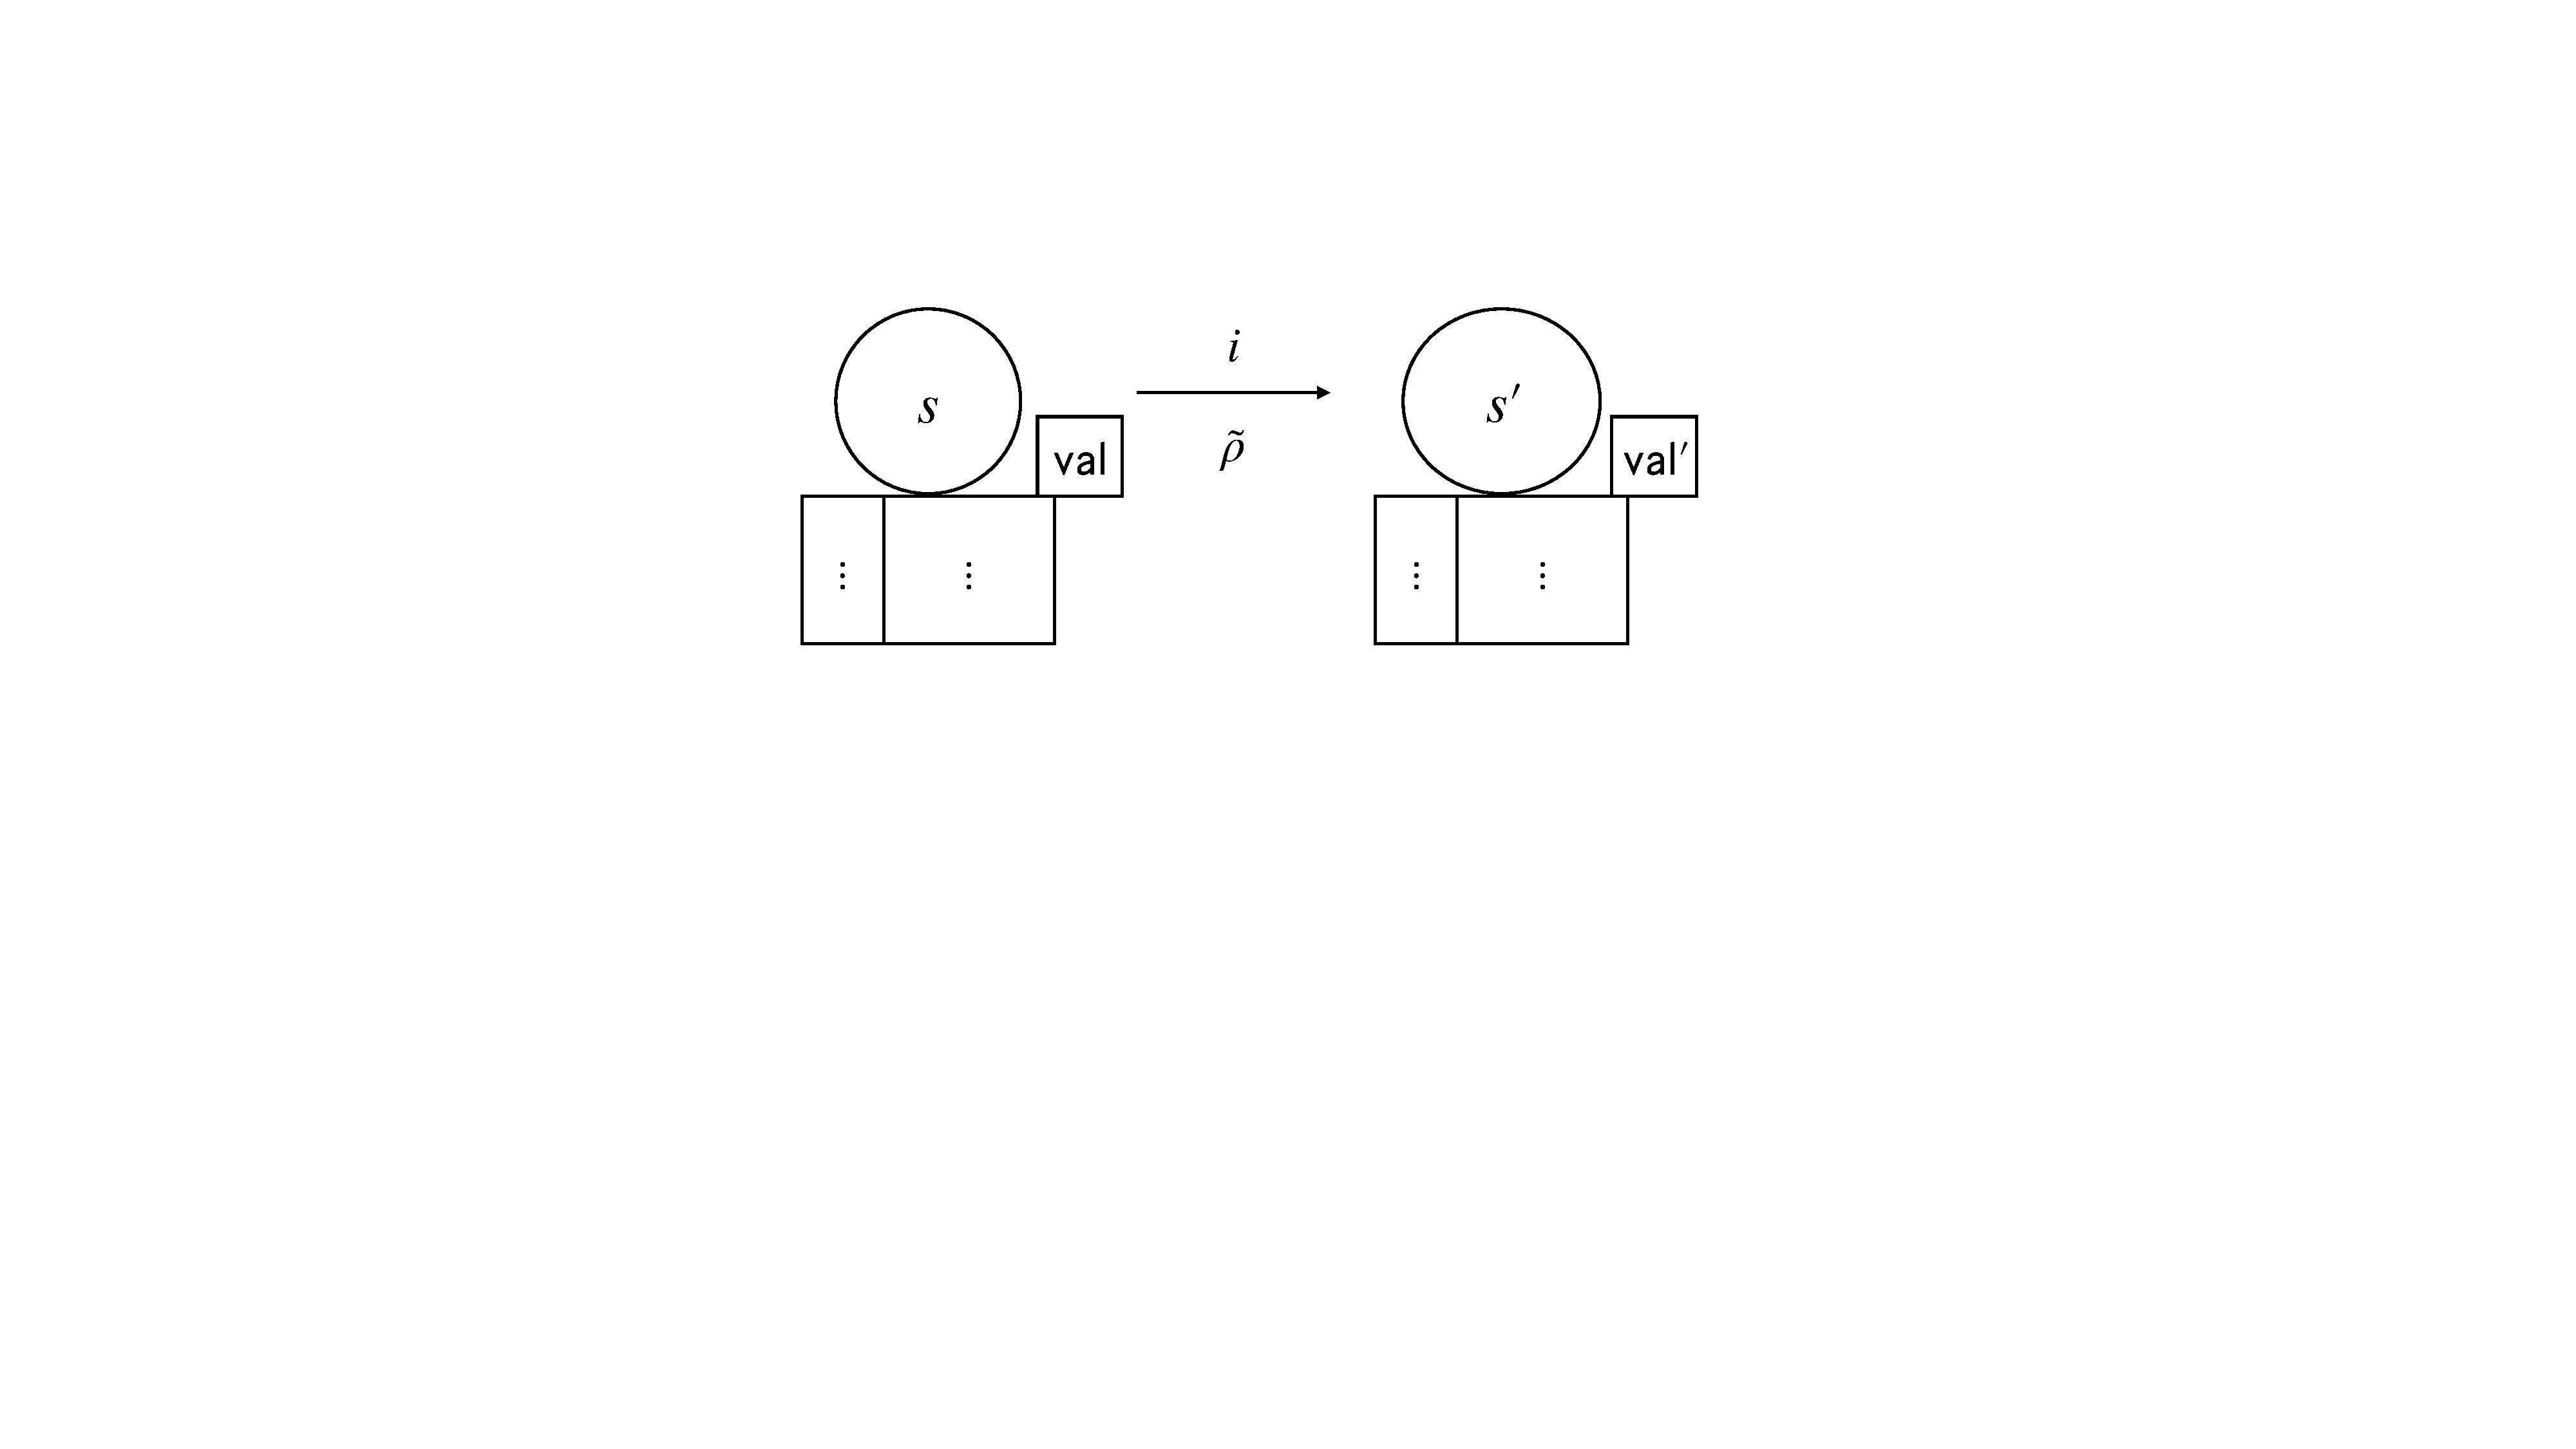
\includegraphics[scale=.2,width=\textwidth/2]{figures/state-transition_cropped.pdf}
  \caption{Transactions representing successive states in a CEM
    transition relation \(\cemStepRel{s}{i}{s'}{\cemTxCon}\).}\label{fig:state-transition}
\end{figure}

%%% Local Variables:
%%% mode: latex
%%% TeX-master: "main"
%%% End:
